\begin{center}
\begin{figure}[ht]
\begin{center}
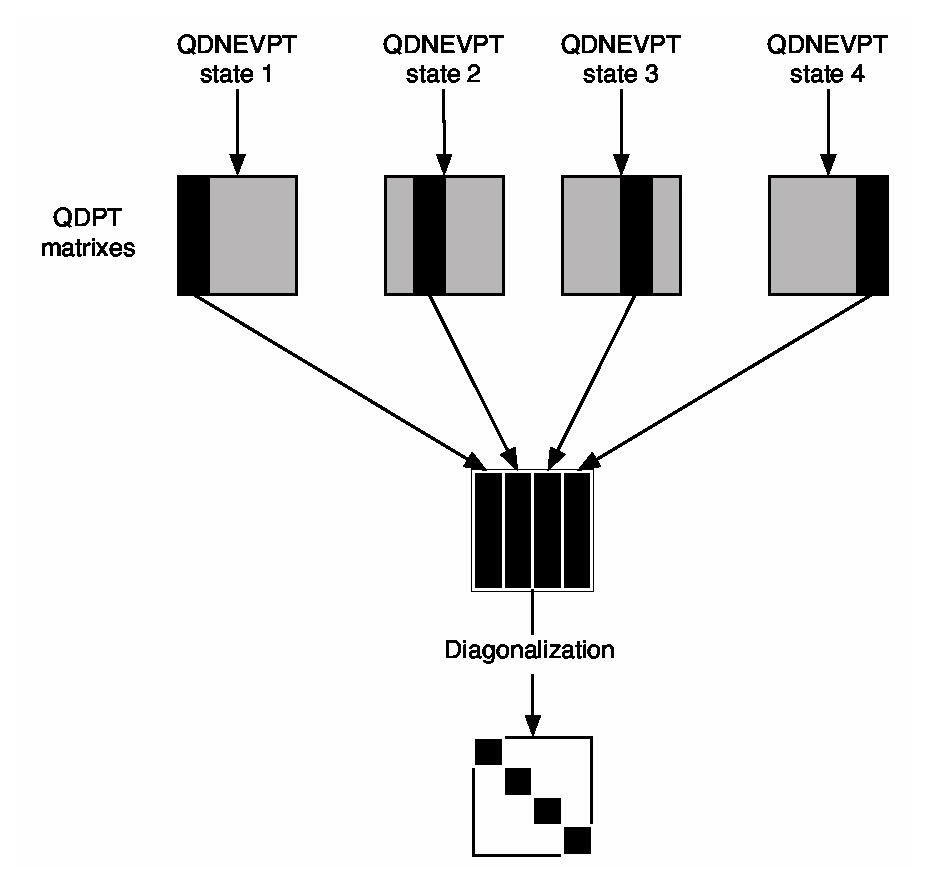
\includegraphics[width=10cm]{03_nevpt/images/qdpt_diagram-gimped.eps}
\end{center}
\caption{\footnotesize The computational scheme for the evaluation of the
Quasi Degenerate treatment. Four different QDPT matrixes are obtained by the
procedure, each one referring to a particular state. A single column is
extracted from each matrix and gathered in a final matrix which is
diagonalized. }
\label{fig:qdpt_diagram}
\end{figure}
\end{center}
